\documentclass[10pt,twocolumn]{article}
\usepackage[letterpaper,hmargin=0.7in,vmargin=0.6in,columnsep=0.25in]{geometry}
\usepackage[T1]{fontenc}
\usepackage{lmodern}
\usepackage{microtype}
\usepackage{amsmath}
\usepackage{booktabs}
\usepackage{graphicx}
\usepackage{xcolor}
\usepackage[hidelinks]{hyperref}
\usepackage{url}
\usepackage{enumitem}
\usepackage{titlesec}
\usepackage{caption}

\setlist{nosep,leftmargin=1.2em}
\titlespacing*{\section}{0pt}{0.7ex plus 0.2ex}{0.4ex}
\titlespacing*{\paragraph}{0pt}{0.4ex}{0.6em}
\titleformat*{\section}{\large\bfseries}
\captionsetup{font=small,labelfont=bf,skip=3pt}
\setlength{\textfloatsep}{8pt plus 2pt}
\setlength{\floatsep}{6pt plus 2pt}
\setlength{\abovedisplayskip}{3pt}\setlength{\belowdisplayskip}{3pt}
\graphicspath{{figs/}}

\title{\vspace{-1.2em}\textbf{Do We Need the Shadow?}\\[0.1em]
  {\large\textbf{Freezing-Aware Weight Versioning for Pipeline-Parallel Training}}\vspace{-0.6em}}
\author{Animesh Jain \qquad Rupankar Podder\\[0.2em]
  \small CS6886 Systems Engineering for Deep Learning \quad
  \small Code: \url{https://github.com/2coolcoder/ShadowFRZ}}
\date{\vspace{-2.2em}}

\begin{document}
\maketitle

\section{Introduction}
When a model is split across $d$ GPUs, plain backpropagation keeps all but one GPU idle:
each stage waits for the gradient from the stage after it. Two families of methods remove this
wait. \emph{Decoupled backpropagation} (DDG~\cite{ddg}) lets every module use a stale error
gradient, so all modules run their backward passes at once. \emph{Pipeline parallelism}
(GPipe~\cite{gpipe}, PipeDream~\cite{pipedream}) keeps $m$ microbatches in flight. Then the
weights change while a microbatch is between its forward and backward pass, so PipeDream
stores up to $d$ weight versions per stage. PipeDream-2BW~\cite{pd2bw} cuts this to two: the
current weights and a \emph{shadow} copy. The price is a uniform one-step delay,
$W^{(t+1)} = W^{(t)} - \nu \nabla f(W^{(t-1)})$.

A separate line of work, \emph{layer freezing} (FreezeOut~\cite{freezeout},
PolicyFRZ~\cite{policyfrz}), stops updating layers that have converged to save compute. Our
idea was to merge the two. Per-layer gradient statistics would decide where 2BW's shadow is
still needed: still-changing layers keep it, slowly changing ones drop it, and converged ones are
frozen. This should save memory without losing accuracy. We asked five questions:
(1)~Does DDG still match backprop against a modern baseline?
(2)~Does BERT need 2BW's shadow at all?
(3)~Does the merge beat 2BW and PolicyFRZ on the models each was evaluated on?
(4)~Which component gives which gain, and is the freezing signal better than chance?
(5)~How do the effects scale from BERT-Mini to BERT-Large?

\section{Prior work}
\textbf{DDG}~\cite{ddg} splits a network into $K$ modules and gives module $k$ error
gradients that are $K{-}k$ steps old. It reports backprop-level accuracy on CIFAR ResNets, but
its backprop baseline uses an older training recipe.
\textbf{PipeDream}~\cite{pipedream} introduced the one-forward-one-backward (1F1B) schedule
and weight stashing. \textbf{PipeDream-2BW}~\cite{pd2bw} double-buffers the weights,
coalesces gradients over $m$ microbatches, and reuses the hyperparameters of synchronous
training. Its paper also describes \textbf{PipeDream-Flush}, which keeps one weight version and
flushes the pipeline every batch; this is the same semantics as GPipe~\cite{gpipe}.
\textbf{FreezeOut}~\cite{freezeout} freezes layers on a fixed schedule.
\textbf{PolicyFRZ}~\cite{policyfrz} freezes a layer when its gradient variation (GV) and
relative magnitude (AM) both fall below thresholds.
Related systems drop weight stashing with learning-rate corrections (PipeMare~\cite{pipemare})
or remove frozen layers from a GPipe pipeline (PipeTransformer~\cite{pipetransformer}). Neither
studies how freezing interacts with 2BW's two weight versions.
For models we use CIFAR ResNets~\cite{resnet} with a modern recipe~\cite{cifarrecipe}, and
BERT~\cite{bert} in the compact sizes of~\cite{turc} with the Pre-LN layout of
Megatron-LM~\cite{megatron}.

\section{Idea and implementation}
\paragraph{Variants.} All variants share one 1F1B engine and differ only in which weight version
each stage uses. We compare
\textbf{vanilla} (Flush semantics, 1 copy, no staleness) and \textbf{2BW} (2 copies) with:
\textbf{1BW}, i.e.\ 2BW with the shadow removed (1 copy);
\textbf{FRZ}, the PolicyFRZ rule alone;
\textbf{2BW-Sel}, which drops the shadow per layer where AM is low;
\textbf{2BW+FRZ}; and \textbf{Full}, our merge (Sel + FRZ).
Three controls test whether the signal matters: freezing random layers on the same budget, a fixed
FreezeOut schedule, and resetting Adam's state when a layer is unfrozen.
In 1BW the update is applied in place, so only microbatches that are in flight during an update
see different weights in forward and backward. On stage $s$ this is a fraction $(d{-}s)/m$ of
microbatches; all others are fresh.

\paragraph{Freezing rule.} Over windows of 100 steps we compute GV and AM per layer. A layer is
frozen if $\text{GV}{<}\theta_1$ and $\text{AM}/\text{AM}_\text{ref}{<}\theta_2$, and its
shadow is dropped if $\text{AM}/\text{AM}_\text{ref}{<}0.8$. Decisions are made only at
weight-version boundaries and not in the first 10\% of training. Frozen layers are thawed and
re-measured every 4 windows. We set the thresholds once, from the vanilla runs, before any
freezing run: $\theta_1{=}0.3$, with $\theta_2{=}0.5$ for ResNet and $0.6$ for BERT.

\paragraph{Exact emulation on 2 GPUs.} The weight version a stage uses depends only on
$(d, m, \text{schedule})$, not on the number of devices. Our \texttt{pipeemu} library builds a
version table $(s,k)\mapsto(v_F,v_B)$ from a 1F1B simulator. It then runs the whole
$d$-stage pipeline on one GPU, copying version $v_F$ into the weights in place before each
forward pass and $v_B$ before each backward pass. This requires fp32/TF32, since mixed
precision would hide the mismatch. Three checks validate the emulator. Vanilla equals
gradient accumulation exactly. 2BW matches its closed-form update to within
$6\times10^{-17}$. A real 2-GPU pipeline (\texttt{torchrun}) matches the emulator bit for bit
for Flush, 2BW and 1BW, and its measured cost of the extra weight copy (2BW $-$ vanilla,
36.3\,MB on stage 1) matches our memory model.
All other memory figures are modelled from per-layer profiles. Each stage stores
$\text{versions}\cdot W + \text{grads} + \text{optimizer state} + (d{-}s{+}1)\cdot\text{activations}$.
Time per batch comes from the 1F1B simulator, with fixed partitions for each model.

\paragraph{Experiments.} All runs use $d{=}m{=}4$ unless noted ($\approx$44\,h on two GPUs).
\textbf{Track A:} DDG with $K\in\{1,2,4\}$ on ResNet-56/110, CIFAR-10/100 (17 runs).
\textbf{Track B:} ResNet-50 on CIFAR-10 for 160 epochs, PolicyFRZ's setting (18 runs).
\textbf{Track C:} Pre-LN BERT Mini/Small/Medium/Base, masked-language-model (MLM)
pre-training on WikiText-103~\cite{wikitext} for 20k steps (31 runs, plus 31 learning-rate sweep
runs), and SST-2 fine-tuning from GLUE~\cite{glue}, from our checkpoints and from the public
\texttt{bert-base}/\texttt{bert-large} checkpoints (36 runs).
All variants reuse the vanilla hyperparameters, as 2BW prescribes.

\section{Evaluation against the baselines}
\paragraph{DDG vs.\ modern backprop (Q1).} With our modern recipe, backprop reaches 94.22\%
on ResNet-56/CIFAR-10, against 93.12\% in the DDG paper. With DDG's own recipe we get 92.81\%,
so the weaker baseline comes entirely from the recipe. $K{=}2$ stays within 0.1--0.25 points
of backprop on CIFAR-10 but loses 0.57 on ResNet-56/CIFAR-100. $K{=}4$ is below backprop in
every configuration, by 0.13 to 1.62 points.

\paragraph{The shadow is what makes 2BW stale (Q2).} On ResNet-50 (Table~\ref{tab:b}), 2BW
is 14 points behind vanilla at epoch 4 (two-seed means: 56.1\% vs.\ 69.8\%; 1BW 69.5\%) and
still trails by 0.23 at the end. 1BW ends at 95.84\%. In BERT pre-training (Table~\ref{tab:c},
Fig.~\ref{fig:mm}), 1BW closes 78\%, 64\% and 50\% of 2BW's loss gap for Mini, Small and
Medium. Each size uses the largest swept rate at which 2BW still trains; for Mini (1e-3) 2BW's
own optimum is 5e-4, so the Mini figure may overstate the gain. On Medium at fixed global batch, the gap tracks the predicted mismatch fraction. At
$m/d{=}4$ only 11\% of microbatches are mismatched and 1BW is within 0.01 of vanilla. Dropping
the shadow also saves 5--8\% of stage-1 memory on BERT. Running 2BW for only the first 10\% of
training keeps most of the gap: the early phase decides the outcome.
The delay also narrows the usable learning rate. At learning rates where vanilla trains, both
2BW and 1BW on Post-LN BERT-Mini stay stuck at a loss of 7.24; this is why we use Pre-LN.

\begin{table}[t]
  \centering\footnotesize
  \setlength{\tabcolsep}{3pt}
  \begin{tabular}{lcccc}
    \toprule
    ResNet-50, C10 & Acc.\ (\%) & $\Delta$ van. & Mem.\textsuperscript{a} & Saved\textsuperscript{b} \\
    \midrule
    Vanilla (2 seeds) & 95.62$\pm$.09 & -- & $-0.1\%$ & -- \\
    2BW (2 seeds) & 95.39$\pm$.01 & $-0.23$ & -- & -- \\
    \textbf{1BW} (2 seeds) & \textbf{95.84}$\pm$.14 & $+0.22$ & $-0.1\%$ & -- \\
    FRZ only & 95.81 & $+0.19$ & $-9.0\%$ & 4.0\% \\
    2BW-Sel & 95.14 & $-0.48$ & 0\% & -- \\
    \textbf{Full (ours)} (2 seeds) & 95.52$\pm$.14 & $-0.10$ & $-8.6\%$ & 3.6--4.6\% \\
    Full, random layers & 95.51 & $-0.11$ & $-8.5\%$ & 3.9\% \\
    Full, FreezeOut sched. & 95.34 & $-0.28$ & $-46.3\%$ & 18.7\% \\
    Full, aggressive thr. & 94.68 & $-0.94$ & -- & 8.4\% \\
    \bottomrule
  \end{tabular}
  \caption{Track B, ResNet-50 on CIFAR-10. \textsuperscript{a}Average stage-1 memory vs.\
    2BW, from the memory model. \textsuperscript{b}Training compute (forward + backward) saved
    by freezing.}
  \label{tab:b}
\end{table}

\begin{table}[t]
  \centering\small
  \setlength{\tabcolsep}{4.5pt}
  \begin{tabular}{lcccc}
    \toprule
    MLM val.\ loss (lr) & Vanilla & 2BW & \textbf{1BW} & Full \\
    \midrule
    Mini (1e-3) & 3.250 & 3.492 & \textbf{3.303} & 3.509 \\
    Small (5e-4) & 2.859 & 3.010 & \textbf{2.914} & 3.020 \\
    Medium (5e-4) & 2.770 & 3.001 & \textbf{2.886} & 3.029 \\
    Base (1e-4) & 2.982 & 3.093 & -- & 3.104 \\
    \bottomrule
  \end{tabular}
  \caption{Track C, Pre-LN BERT pre-training, 20k steps. Medium vanilla, 2BW and Full are
    2-seed means (seed noise $\pm$0.03).}
  \label{tab:c}
\end{table}

\begin{figure}[t]
  \centering
  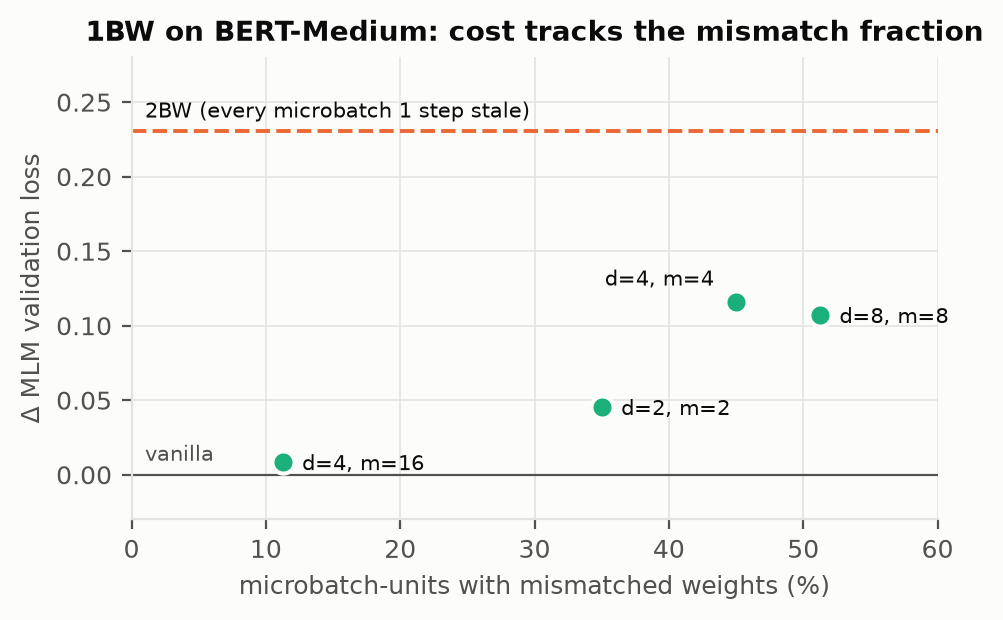
\includegraphics[width=0.74\linewidth]{mismatch_vs_gap.png}
  \caption{BERT-Medium, global batch 128. 1BW's loss gap to vanilla shrinks with the fraction
    of mismatched microbatches. 2BW's gap does not depend on $d$.}
  \label{fig:mm}
\end{figure}

\paragraph{The merge vs.\ 2BW and PolicyFRZ (Q3, Q4).} In pre-training, Full is within noise of
2BW: $+0.13$ points on ResNet-50 and $+0.028$ loss on BERT-Medium. The ablations explain why.
Removing \emph{all} shadows (1BW) gives the accuracy gain. Removing them \emph{selectively} keeps
the shadows early in training, exactly when they hurt. Freezing gives the memory gain
($-8.6\%$ stage-1 memory, $-4\%$ time per batch on ResNet-50).
On ResNet-50 the GV/AM signal does no better than freezing random layers on the same budget.
PolicyFRZ reports $\sim$28\% compute savings against a 92.0\% baseline. On the same model, our
baseline is 3.6 points stronger (95.62\%), and the PolicyFRZ rule saves only $\sim$4\%; forcing
earlier freezing costs 0.94 points. During pre-training GV stays near the noise
level for every layer, so ``GV low and AM low'' only holds in the low-learning-rate tail.

\paragraph{Fine-tuning (Q3).} Fine-tuning is the setting PolicyFRZ targets: gradients shrink
as the task is learned, so the rule fires often. Starting from the public checkpoints on SST-2,
Full freezes 24--26\% of layer-windows (Table~\ref{tab:ft}). It uses 15.6\% less stage-1 memory
than 2BW on BERT-Large and is the most accurate variant there. On BERT-Base it saves 12.9\% but
is about 1 point below 2BW. Each entry is one run on the 872-example dev set, where one standard
error is about 0.9 points.

\begin{table}[h]
  \centering\footnotesize
  \setlength{\tabcolsep}{3.5pt}
  \begin{tabular}{lccccc}
    \toprule
    SST-2 acc.\ (\%) & Vanilla & 2BW & Full & Mem.\ vs.\ 2BW & Frozen \\
    \midrule
    BERT-Base & 92.32 & 92.55 & 91.51 & $-12.9\%$ & 26\% \\
    BERT-Large & 93.35 & 93.81 & 94.38 & $-15.6\%$ & 24\% \\
    \bottomrule
  \end{tabular}
  \caption{SST-2 fine-tuning, public checkpoints, 1 epoch. Memory: average stage 1, modelled.}
  \label{tab:ft}
\end{table}

\paragraph{Scaling (Q5).} At a fixed learning rate, 2BW's gap grows with depth: $+0.15$ on
Small, $+0.23$ on Medium. 1BW's advantage shrinks with more stages at fixed $m/d$ and comes back
with larger $m/d$.

\paragraph{Limitations.} Memory and time for $d{>}2$ are modelled. Only the weight-copy memory
was measured on real hardware, so activation memory and the freezing savings are modelled only.
Most rows have one seed (two for key rows). Pre-training covers only the first 20k steps.

\paragraph{Conclusion.} 2BW's shadow causes its staleness: removing it uses less memory, trains
better, and is close to exact at $m/d\ge4$. PolicyFRZ's statistics did not find converged layers
in pre-training. In fine-tuning the merge saves 13--16\% of stage-1
memory, with the best accuracy on BERT-Large and about 1 point less on BERT-Base.

\label{lastbodypage}

{\small
\begin{thebibliography}{99}\setlength{\itemsep}{0pt}
\bibitem{ddg} Z.~Huo, B.~Gu, Q.~Yang, H.~Huang. Decoupled Parallel Backpropagation with Convergence Guarantee. \emph{ICML}, 2018. \url{https://proceedings.mlr.press/v80/huo18a.html}
\bibitem{pipedream} D.~Narayanan, A.~Harlap, A.~Phanishayee, V.~Seshadri, N.~R.~Devanur, G.~R.~Ganger, P.~B.~Gibbons, M.~Zaharia. PipeDream: Generalized Pipeline Parallelism for DNN Training. \emph{SOSP}, 2019. \url{https://doi.org/10.1145/3341301.3359646}
\bibitem{pd2bw} D.~Narayanan, A.~Phanishayee, K.~Shi, X.~Chen, M.~Zaharia. Memory-Efficient Pipeline-Parallel DNN Training. \emph{ICML}, 2021. \url{https://proceedings.mlr.press/v139/narayanan21a.html}
\bibitem{gpipe} Y.~Huang et al. GPipe: Efficient Training of Giant Neural Networks using Pipeline Parallelism. \emph{NeurIPS}, 2019. \url{https://arxiv.org/abs/1811.06965}
\bibitem{freezeout} A.~Brock, T.~Lim, J.~M.~Ritchie, N.~Weston. FreezeOut: Accelerate Training by Progressively Freezing Layers. arXiv:1706.04983, 2017. \url{https://arxiv.org/abs/1706.04983}
\bibitem{policyfrz} L.~Gao, S.~Han, X.~Wang, X.~Wang, Z.~Zou, L.~Jiang. PolicyFRZ: Adaptive Layer Freezing via Policy Networks for Accelerating DNN Training in Edge Environments. \emph{Intelligent and Converged Networks}, 7(3), 2026. \url{https://ieeexplore.ieee.org/abstract/document/11701677}
\bibitem{pipemare} B.~Yang et al. PipeMare: Asynchronous Pipeline Parallel DNN Training. \emph{MLSys}, 2021. \url{https://arxiv.org/abs/1910.05124}
\bibitem{pipetransformer} C.~He, S.~Li, M.~Soltanolkotabi, S.~Avestimehr. PipeTransformer: Automated Elastic Pipelining for Distributed Training of Transformers. \emph{ICML}, 2021. \url{https://arxiv.org/abs/2102.03161}
\bibitem{resnet} K.~He, X.~Zhang, S.~Ren, J.~Sun. Deep Residual Learning for Image Recognition. \emph{CVPR}, 2016. \url{https://arxiv.org/abs/1512.03385}
\bibitem{cifarrecipe} Y.~Chen. PyTorch CIFAR models (ResNet-56 training recipe). \url{https://github.com/chenyaofo/pytorch-cifar-models}
\bibitem{bert} J.~Devlin, M.-W.~Chang, K.~Lee, K.~Toutanova. BERT: Pre-training of Deep Bidirectional Transformers for Language Understanding. \emph{NAACL}, 2019. \url{https://arxiv.org/abs/1810.04805}
\bibitem{turc} I.~Turc, M.-W.~Chang, K.~Lee, K.~Toutanova. Well-Read Students Learn Better: On the Importance of Pre-training Compact Models. arXiv:1908.08962, 2019. \url{https://arxiv.org/abs/1908.08962}
\bibitem{megatron} M.~Shoeybi et al. Megatron-LM: Training Multi-Billion Parameter Language Models Using Model Parallelism. arXiv:1909.08053, 2019. \url{https://arxiv.org/abs/1909.08053}
\bibitem{wikitext} S.~Merity, C.~Xiong, J.~Bradbury, R.~Socher. Pointer Sentinel Mixture Models (WikiText-103). \emph{ICLR}, 2017. \url{https://arxiv.org/abs/1609.07843}
\bibitem{glue} A.~Wang et al. GLUE: A Multi-Task Benchmark and Analysis Platform for Natural Language Understanding. \emph{ICLR}, 2019. \url{https://arxiv.org/abs/1804.07461}
\bibitem{code} A.~Jain, R.~Podder. ShadowFRZ: code, results and reproduction scripts for this project. \url{https://github.com/2coolcoder/ShadowFRZ}
\end{thebibliography}
}
\end{document}
